%==============================================================================
% BYOP Machine Vision Camera -- press release
% DRAFT. See NOTES FOR REVIEW at the end of this file before distribution.
%==============================================================================
\documentclass[11pt]{article}

\usepackage[letterpaper,margin=1in]{geometry}
\usepackage{graphicx}
\usepackage{caption}
\usepackage{booktabs}
\usepackage{xcolor}
\usepackage{titlesec}
\usepackage{parskip}
\usepackage[colorlinks=true,urlcolor=ukblue,linkcolor=ukblue]{hyperref}

\definecolor{ukblue}{RGB}{0,51,160}

\titleformat{\section}{\normalfont\large\bfseries\color{ukblue}}{}{0pt}{}
\titlespacing*{\section}{0pt}{12pt}{4pt}

\newcommand{\pressrule}{\textcolor{ukblue}{\rule{\linewidth}{1.2pt}}}

\begin{document}
\pagestyle{empty}

\noindent
\pressrule

\vspace{6pt}
\noindent
\begin{minipage}[t]{0.40\linewidth}
{\bfseries FOR IMMEDIATE RELEASE}
\end{minipage}\hfill
\begin{minipage}[t]{0.56\linewidth}
\raggedleft\small
\textit{Contact:} Daniel L. Lau\\
DataBeam Professor of Electrical and Computer Engineering\\
University of Kentucky\\
\href{mailto:dllau@uky.edu}{dllau@uky.edu}
\end{minipage}

\vspace{18pt}

\begin{center}
  {\LARGE\bfseries University of Kentucky Researchers Develop\\[2pt]
   ``Bring Your Own Projector'' Machine Vision Camera}\\[10pt]
  {\large A single board pairs a conventional industrial camera with a built-in
   HDMI controller,\\ turning any projector into a structured-light 3D scanner
   --- and chaining\\ camera to camera over the video signal itself.}
\end{center}

\vspace{12pt}

\noindent\textbf{LEXINGTON, Ky.} --- Researchers at the University of Kentucky
have introduced a machine vision camera that incorporates an HDMI controller for
interfacing directly to commodity projectors. The board is a traditional high-speed
machine vision camera --- a global-shutter
sensor streaming full frames over USB~3.0 --- with a complete HDMI receiver and
transmitter integrated alongside it on the same FPGA. Video from a host computer
enters the camera and passes through to a projector. Because the camera sits
\emph{in} the video path rather than beside it, it knows precisely what is being
projected, and when.

The team calls the result BYOP, for \emph{Bring Your Own Projector}: connect any
HDMI projector and the system becomes a structured-light 3D scanner, with no
external trigger box, frame grabber, or custom synchronization cabling. The reason to
want that is access. Structured-light systems are conventionally built around dedicated
projection light engines --- metrology modules made in small volumes, at prices that
dominate the cost of the instrument. To an industrial buyer specifying a measuring
machine, that cost is simply part of the machine. To everyone else it is a barrier, and
it has confined structured-light 3D scanning to the groups that can afford the light
engine.

Academic laboratories, this one included, have long worked the other way round
--- adapting to the commodity projectors they can actually buy. Those projectors are
mass-produced against the 3D-Ready and DLP market, and they bring real advantages of
their own: high luminance, a wide choice of fields of view and throw distances, and,
with LED illumination, an operating life measured in tens of thousands of hours. What
has made them awkward to build with was never their optics --- it was the difficulty of
making a camera keep time with a device never designed to be part of a measuring
instrument.

The instrument is built as a stack. Three of its boards are commercially available
parts from \textbf{Alchitry} --- the Pt~V2 mainboard carrying the Artix-7 FPGA, the
Ft+ for the USB~3.0 link, and the Hd+ for HDMI in and out --- and on top of them sits
a \textbf{custom-designed sensor board}, developed for this project, carrying the
PYTHON~1300 and its power supplies. The boards mate through a common high-density
stacking connector, so the whole camera assembles without a single internal cable and
drops into the printed enclosure shown in Figure~\ref{fig:stack}.
Table~\ref{tab:hardware} summarises the hardware.

\section{Why put HDMI inside a camera?}

Structured-light 3D scanning works by projecting a sequence of patterns onto an
object and photographing each one. The measurement is only as good as the
synchronization: the camera must expose once per projected pattern, at a known
moment within that pattern's display time. Conventionally, that means a trigger
generator, a cable harness, and a calibration step for the delay between them ---
an assembly that has to be reworked whenever the projector, the frame rate, or the
pattern set changes. Integrating the video interface into the camera removes the
problem rather than managing it. The projected frames and the camera's exposures
come from the same signal, inside one device.

It also solves a subtler problem. A PC's graphics hardware is not a real-time
system: it may hold the same image on screen for an extra refresh, or deliver the
next one late, and nothing in the video signal announces which has happened. The
camera therefore reads the \textbf{top-left pixel} of every incoming frame and
watches that value for change. A change means a genuinely new pattern has arrived
and the frame should be captured; no change means the computer has repeated itself
and the frame should be ignored. That sampled value then travels with the image:
it is embedded in the \textbf{frame header} the camera sends to the host, so the PC
can line the sequence of captured frames up against the sequence of patterns it
played. The pattern sequence and the captured sequence stay in step even though the
machine driving them makes no timing guarantees.

\section{The imager}

The camera is built around the \textbf{onsemi PYTHON 1300}, a global-shutter CMOS
sensor with $1280 \times 1024$ resolution --- 1.3 megapixels --- reading out over
four LVDS channels at 720\,Mbit/s each. The sensor is socketed, and the same board
accepts either the \textbf{monochrome or the colour} variant of the part. Its
pixels are 4.8\,$\mu$m square, with a \textbf{global shutter}, and are delivered at
\textbf{10 bits} of depth --- 1024 grey levels rather than 256. At full resolution
and 10-bit depth the sensor is capable of \textbf{210 frames per second}. For live
streaming, the camera delivers \textbf{120 frames per second} over its USB-C
connection, at the sensor's full $1280 \times 1024$ and full 10-bit depth --- no
cropping, no windowing, and no reduction in depth. For slower USB~2.0 connections,
the camera does not have to stream at all. Frames are captured into \textbf{on-board
DDR3 memory} as they are projected and downloaded afterwards, so the speed of the
scan is set by the HDMI frame rate rather than by the streaming rate of the host
connection.

\section{No host HDMI source required}

The camera does not have to be fed video at all. The board generates its own
pattern sequences internally and drives the projector directly, at frame rates up
to \textbf{120 per second} --- the same rate at which it streams full frames. That
rate is not arbitrary. \textbf{3D-Ready DLP projectors} --- a large and inexpensive
installed base, built to accept 120\,Hz for shutter-glasses stereo --- take a
120\,Hz signal as a matter of course. The camera drives them at their native rate,
and the highest standard mode it drives at 120\,Hz is \textbf{800$\times$600}. The
entire structured-light loop --- project a pattern, capture it, advance to the next
--- therefore runs on the camera itself, at 120\,Hz, with nothing driving the video
path but the camera. A computer is needed only to collect the resulting images, not
to generate what is projected.

Where a host \emph{is} driving the display, the FPGA can be configured to work
either way. It can \textbf{replace} the incoming pixels with its own structured-light
scan patterns, generated to suit the resolution arriving on the cable, and trigger
the camera on every vertical sync --- the host supplies the video timing, the camera
supplies the patterns. Or it can \textbf{pass} the host's pixels through untouched
and use the top-left-pixel mechanism to decide when to trigger, leaving the pattern
sequence entirely to the software driving the display. The same hardware serves
both arrangements.

\section{Any projector --- and a host offered only what works}

Nothing about the camera is tied to a particular projector, or to a particular
projection technology. On power-up it reads the connected projector's \textbf{EDID}
--- the data block every display serves back over the video cable, listing the
resolutions and frame rates it will accept --- and adapts to whatever it finds there.
DLP, LCD or LCoS, the camera drives the projector at a mode that projector itself
advertises, rather than at an assumed one. The 120\,Hz 3D-Ready projectors described
above are simply the fastest case, not a requirement.

When a host PC is in the video path, the camera goes a step further: it builds an EDID
of its own and serves that to the computer, offering the projector's own mode list
narrowed to those modes the camera can also receive. The PC is therefore shown a set
of display modes already known to work end to end, and the operator chooses among them
in the ordinary display settings.

Nothing in that arrangement is specific to projectors, and the group expects to put it
to work on high-speed gaming monitors next. Displays running at \textbf{200 to
210\,Hz} are now commodity items, and at those rates a screen meets the PYTHON 1300 at
the top of its own range --- 210 frames per second. The application is
\emph{deflectometry}, where the pattern is reflected off a specular surface rather
than projected onto a diffuse one, and where shiny parts that defeat a projector are
exactly the ones worth measuring. That is intended future work, not a capability of
the board today.

\section{Daisy-chaining: one video signal, many cameras}

Because the HDMI path runs \emph{through} the camera --- a separate input and output
port, visible in Figure~\ref{fig:connectors} --- cameras can be chained. The host
drives the first unit; each unit forwards the video onward to the next and, finally,
to the projector. Every camera in the chain sees the same frames and can key to them.

That makes multi-camera geometries straightforward to assemble:

\begin{itemize}\itemsep2pt
  \item \textbf{Active stereo} --- two or more cameras viewing a
        projector-illuminated scene, capturing the same pattern from different
        viewpoints.
  \item \textbf{Multi-view capture} --- cameras arranged around a subject, all
        keyed to a common projected sequence.
  \item \textbf{Extended baselines} --- units placed far apart, coordinated over
        the same cable that already carries the video.
\end{itemize}



\section{Background --- the work this camera comes from}

The architecture announced here was proposed and argued for in this group's earlier
published work. What is new is that it has been built, and measured. Readers who want
the reasoning behind the design will find it in the following.

\begin{itemize}\itemsep4pt
  \item M.~P.~Ruffner, Y.~Yu and D.~L.~Lau, ``Structured light smart camera for spatial
        augmented reality applications,'' \emph{Proc. SPIE} \textbf{10932}, Emerging
        Digital Micromirror Device Based Systems and Applications XI, 109320J (2019).
        \href{https://doi.org/10.1117/12.2508553}{doi:10.1117/12.2508553}\\
        \small\textit{The direct predecessor. It sets out why a PC cannot be trusted to
        synchronize a projector and a camera, and proposes putting the image sensor and
        an HDMI input and output onto the FPGA controller itself --- the design this
        camera realizes.}
  \item M.~P.~Ruffner, ``Design of a Machine Vision Camera for Spatial Augmented
        Reality,'' MSEE thesis, University of Kentucky (2018).
        \href{https://uknowledge.uky.edu/ece_etds/129/}{uknowledge.uky.edu/ece\_etds/129}\\
        \small\textit{The long-form treatment of the same design, including the power
        and layout work that a sensor board of this kind stands or falls on.}
  \item Y.~Yu, D.~L.~Lau, M.~P.~Ruffner and K.~Liu, ``Dual-projector structured light 3D
        shape measurement,'' \emph{Applied Optics} \textbf{59}(4), 964--974 (2020).
        \href{https://doi.org/10.1364/AO.378363}{doi:10.1364/AO.378363}\\
        \small\textit{Why more than one light engine is worth the trouble: fewer
        occlusions, better signal-to-noise, fewer frames per scan, and multi-path
        made visible. The argument that makes a chainable camera worth building.}
  \item Y.~Yu and D.~L.~Lau, ``3D scanning by means of dual-projector structured light
        illumination,'' \emph{Proc. SPIE} \textbf{10932}, 109320M (2019).
        \href{https://doi.org/10.1117/12.2510990}{doi:10.1117/12.2510990}\\
        \small\textit{The conference treatment of the above, with the temporal-frequency
        multiplexing that lets two projectors run at once.}
\end{itemize}

\vfill

\begin{quote}
\itshape
``This system is the culmination of years of research and development into structured
light imaging, and by making commodity projector synchronization so easy, I hope it
unlocks years more of technological improvements in SLI.''
\end{quote}

\noindent --- Daniel L. Lau, DataBeam Professor of Electrical and Computer
Engineering, University of Kentucky

\vfill

\section{About}

The BYOP camera comes out of the laboratory of \textbf{Daniel L. Lau}, DataBeam
Professor of Electrical and Computer Engineering at the University of Kentucky, whose
career in three-dimensional imaging spans twenty-five years. Since joining the
University of Kentucky in 2001, he has worked on structured-light 3D imaging --- both
the algorithms that make real-time, high-accuracy shape measurement possible and the
instruments that have to carry them --- work that established non-contact 3D
fingerprint capture as a practical alternative to contact scanning and that has reached
industry through two companies he co-founded, FlashScan3D and Seikowave. He is also a
pioneer of digital halftoning, and in 2026 was elected a Fellow of the IEEE for
contributions to digital printing and 3D imaging.

\vspace{6pt}
\pressrule
\begin{center}\small \#\ \#\ \#\end{center}

\clearpage
\clearpage
\begin{table}[h!]
\centering
\small
\begin{tabular}{@{}ll@{}}
\toprule
\textbf{Image sensor}      & onsemi PYTHON 1300, socketed --- monochrome or colour \\
\textbf{Resolution}        & $1280 \times 1024$ (1.3\,MP), global shutter \\
\textbf{Pixel depth}       & 10 bits per pixel (1024 grey levels); 8-bit selectable \\
\textbf{Sensor frame rate} & 210 frames/s at full resolution, 10-bit \\
\textbf{Streamed rate}     & 120 frames/s sustained over USB-C \\
\textbf{Camera timing}     & Free-running, or keyed to the projector --- HDMI sync not required \\
\textbf{Buffered capture}  & To on-board DDR3 at sensor rate, downloaded after \\
\textbf{Host interface}    & USB 3.0, byte-exact --- 325\,MB/s achieved in testing \\
\textbf{Video in / out}    & HDMI receive and transmit, pass-through \\
\textbf{Projector support} & Reads the projector's EDID; any projector in the window \\
\textbf{Pass-through window} & 25--90\,MHz pixel clock, enforced in the EDID served to the host \\
\textbf{Standalone output} & Board-generated video, no HDMI source needed \\
\textbf{Highest 120\,Hz mode} & 800$\times$600 at 120\,Hz (3D-Ready DLP projectors) \\
\textbf{Verified modes}    & $640\times480$ through $1280\times800$, 60 to 120\,Hz \\
\textbf{Processing}        & Xilinx Artix-7 FPGA with DDR3 frame buffer \\
\textbf{Construction}      & Alchitry Pt~V2, Ft+ and Hd+ boards plus a custom sensor board \\
\textbf{On-board patterns} & Sinusoidal fringe generation, radiometric linearization \\
\bottomrule
\end{tabular}
\caption{\small\textbf{BYOP camera --- hardware summary.}}
\label{tab:hardware}
\end{table}
\clearpage

\clearpage
\begin{figure}[h!]
  \centering
  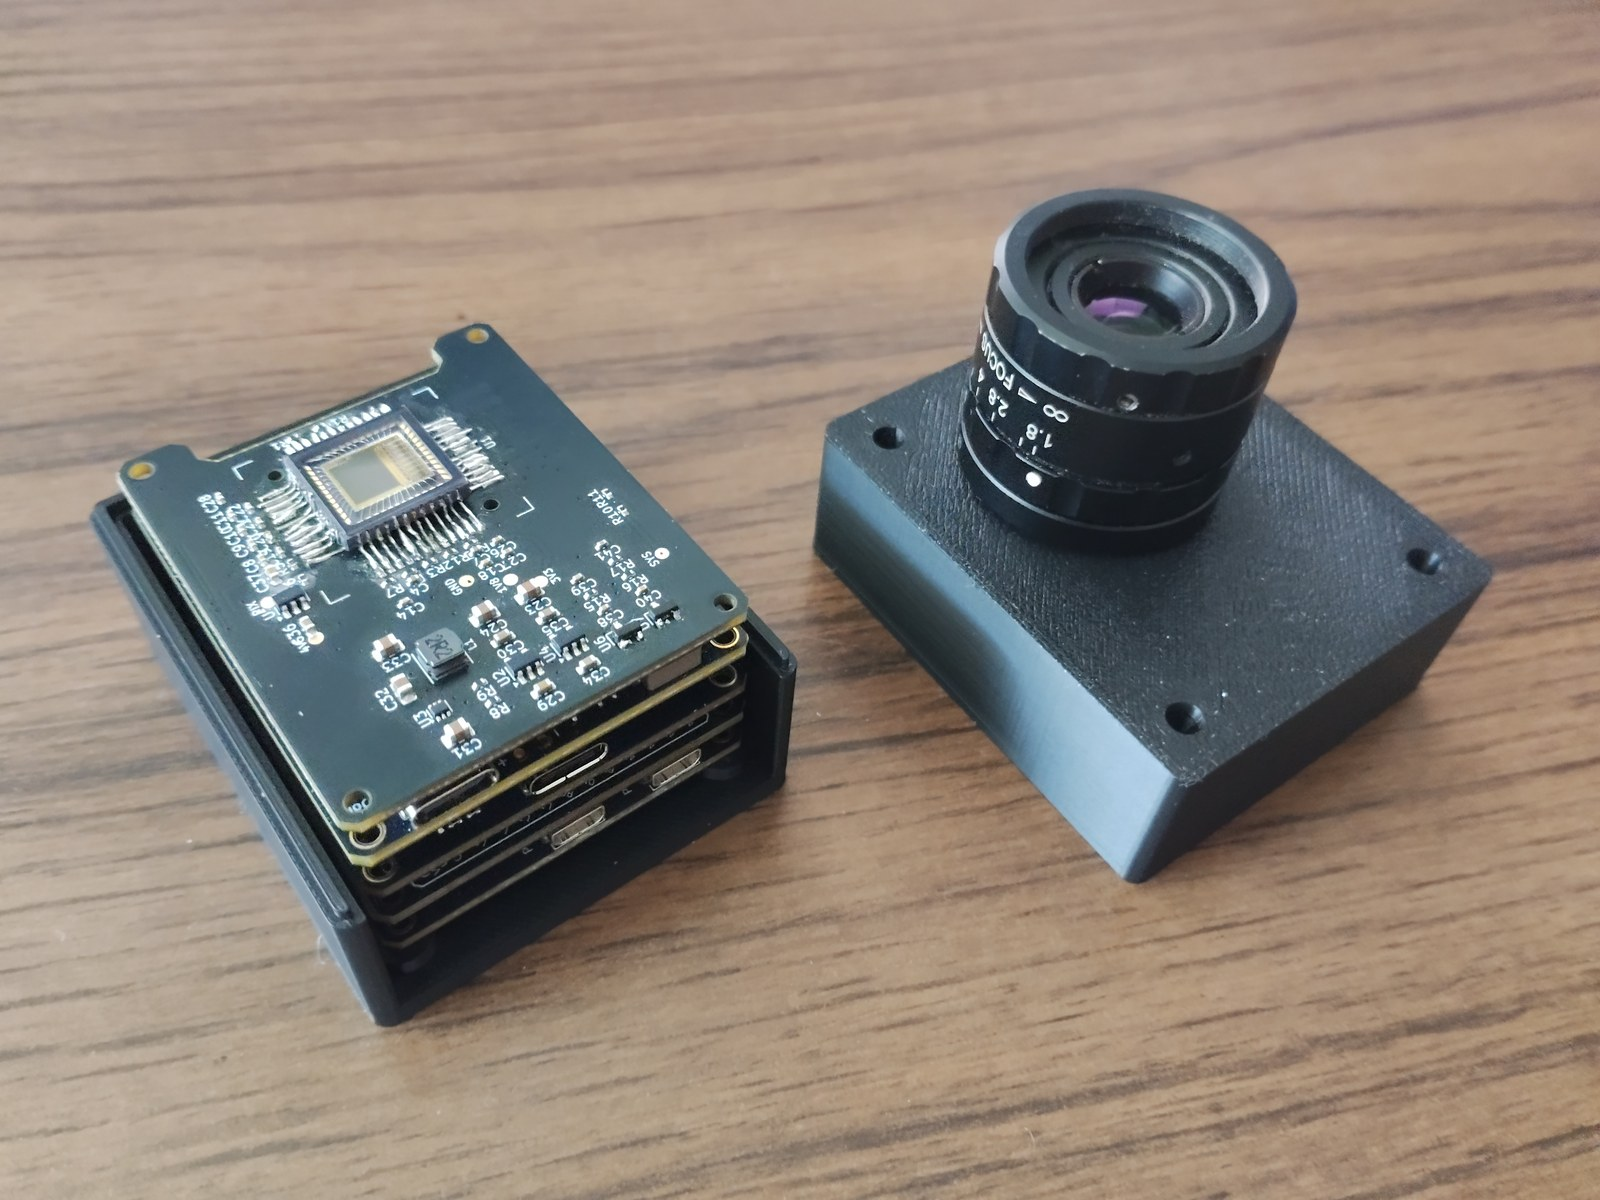
\includegraphics[width=0.70\linewidth]{stack_with_lens_cap_print.jpg}
  \caption{\small\textbf{The complete camera, opened.} The board stack sits in its
  printed enclosure: the HDMI board at the bottom, the USB~3.0 image link and the
  Artix-7 FPGA above it, and the PYTHON~1300 sensor board on top, its glass lid
  facing up. The 48-pin sensor was soldered by hand in
  the lab. At right, the enclosure's lid carries the lens and drops straight onto
  the stack. \textit{Photo: University of Kentucky.}}
  \label{fig:stack}
\end{figure}

\begin{figure}[h!]
  \centering
  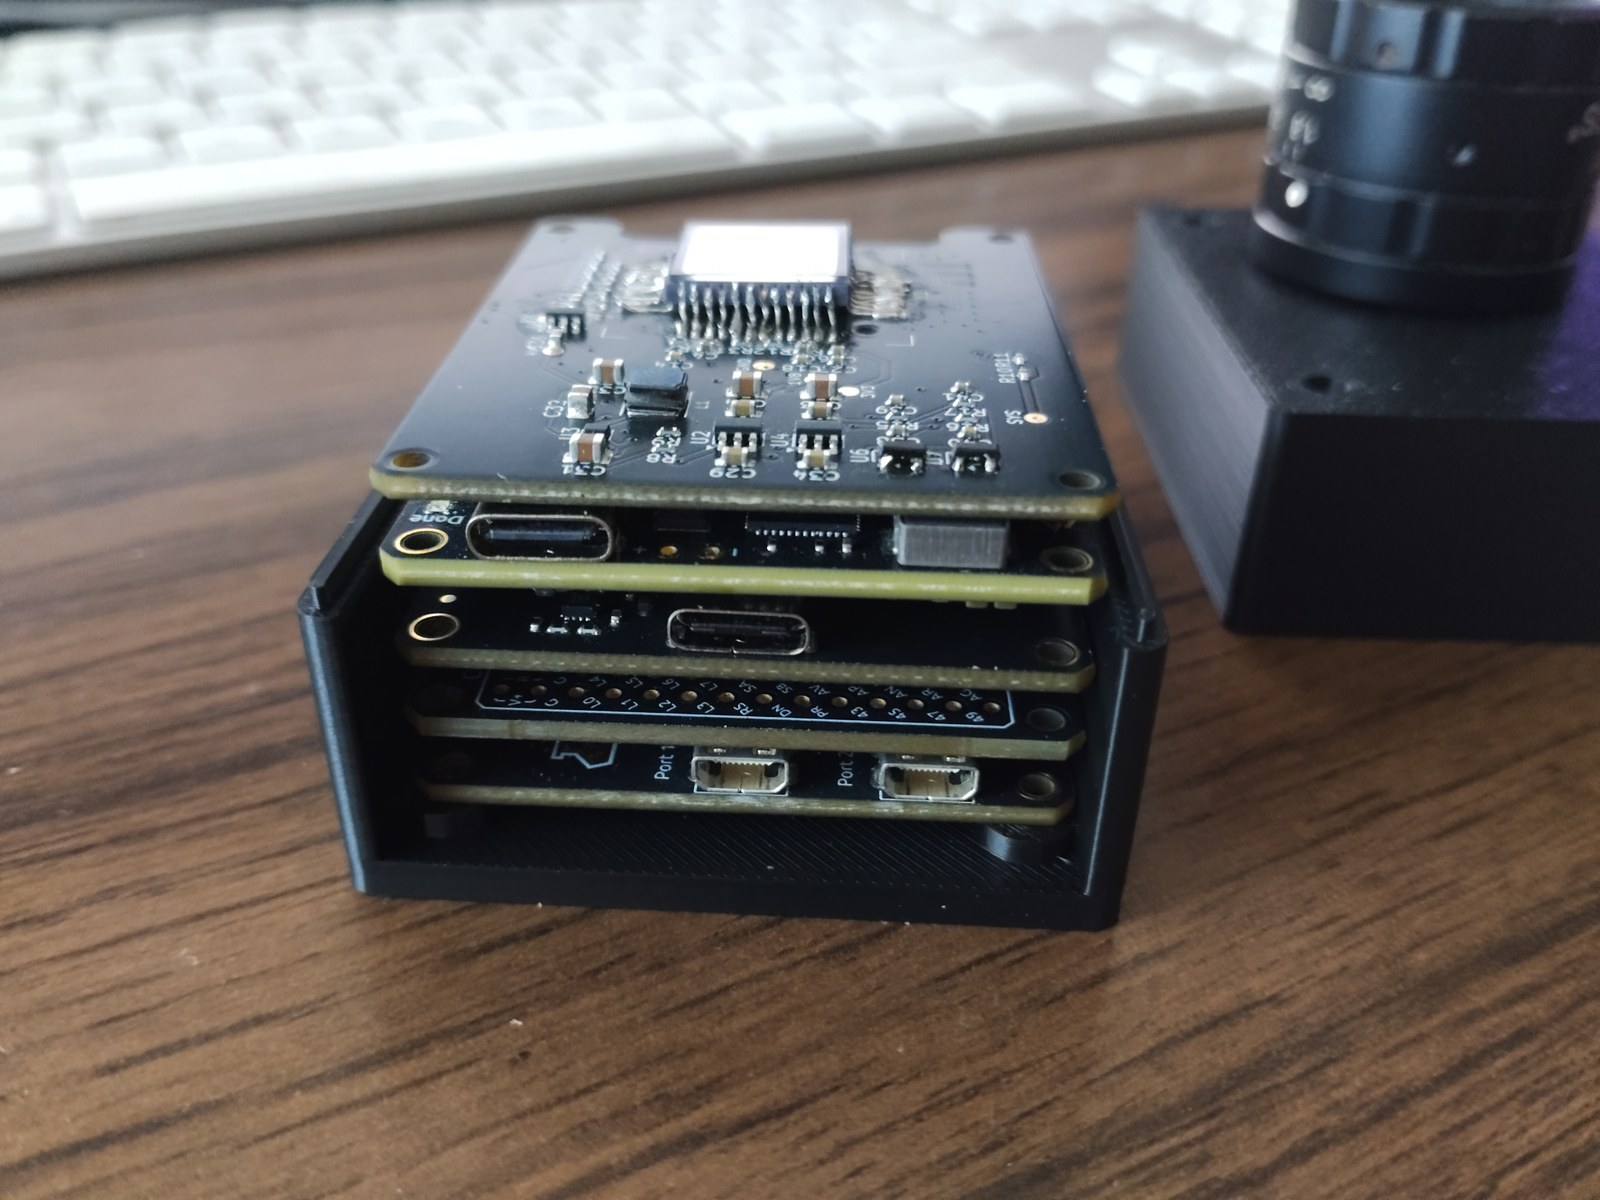
\includegraphics[width=0.70\linewidth]{stack_connector_edge_print.jpg}
  \caption{\small\textbf{The connector edge.} The two HDMI ports at the bottom are
  the video input and output. The \emph{input} is fed by the host PC, or by the
  previous camera when units are daisy-chained; the \emph{output} drives the
  projector, or the next camera in the chain. Above them, the lower USB-C connector
  carries the image stream to the host. The sensor board is the topmost in the stack. \textit{Photo: University of Kentucky.}}
  \label{fig:connectors}
\end{figure}


\end{document}

%==============================================================================
% NOTES FOR REVIEW -- read before this leaves the building
%==============================================================================
%
% MEASURED, SAFE TO STATE AS FACT:
%   * MONO/COLOUR: the part in the socket today is the MONOCHROME NOIP1SN1300A-QTI
%     (P1-SN). The colour variant is a different part number in the same family and
%     package; the board has not been built or tested with one. VERIFY before the
%     release states it as an option -- the claim is electrical/mechanical
%     compatibility, and colour would additionally need host-side demosaicing.
%   * 10-BIT is real and worth leading with: 1024 grey levels vs 256. The sensor
%     runs 10-bit via divide-by-5 clocking (reg 32[3] adc_mode = 0); 8-bit is
%     divide-by-4. Both reach the same 720 Mbps/lane and the same max frame rate,
%     so 10-bit costs nothing in speed -- see CAMERA_SENSOR_PROTOCOL.md 4.0.
%   * SENSOR: onsemi PYTHON 1300 (NOIP1SN1300A-QTI), monochrome, 4 LVDS channels
%     at 720 Mbps. 1280x1024, 8/10-bit, global shutter. 210 fps ZROT at full SXGA
%     (165 fps NROT) -- sourced to CAMERA_SENSOR_PROTOCOL.md, which cites the
%     onsemi datasheet directly.
%   * The 210 fps figure is the SENSOR's; 120 fps is what the camera SUSTAINS over
%     USB-C at FULL 1280x1024 and full 10-bit depth. Do not collapse them into one
%     number. What makes the full frame fit the link is PACKED 10-bit (10-to-a-word
%     rather than padded into 16); padding costs 37% of the rate for no extra
%     information.
%
%   * DO NOT REINSTATE THE ROI CLAIM. An earlier draft said the sensor's "up to
%     eight simultaneous regions of interest" were how the camera holds 120 fps.
%     BOTH HALVES WERE WRONG and the paragraph has been cut:
%       - NOT IMPLEMENTED. grep for roi|window_id|win_id|roi_id across
%         sources_1/imports/RTL/ and LauPythonCamera_Pt_Stack/ddr/ returns ZERO
%         hits. Nothing configures the sensor's windowing registers and no host
%         tool exposes them. The only mention in the repo is FRAME_HEADER_PLAN.md
%         ("roi_id -- 3 bits. Moves to word 2 IF ROIs are actually used").
%       - WRONG MECHANISM ANYWAY. 120 Hz is achieved at FULL FRAME, no cropping --
%         LauPythonCamera_Pt_Stack/README.md "Operating point -- ACHIEVED
%         2026-08-17", confirmed by the 30-minute M7 soak. No pixels are skipped.
%     What IS true and datasheet-cited is that the PYTHON 1300 SUPPORTS up to 8
%     windows and tags every frame-sync code with a 3-bit window ID (0-7). That is
%     a property of the PART, not a feature of this camera. It is how the earlier
%     draft's notes came to file it under "safe to state as fact". If ROIs are ever
%     built, this claim can come back -- with a measurement behind it.
%   * BUFFER-THEN-DOWNLOAD is the faster path for scans: capture into on-board
%     DDR3 at sensor rate, download afterwards, so scan length is set by the
%     sensor and not the host link. NOTE this describes the SEQUENTIAL mode
%     (capture all frames, then replay), which is the shipping design. OVERLAPPING
%     capture with download -- which would roughly halve scan time again -- was
%     attempted on branch wip/concurrent-capture and DOES NOT WORK (DDR3 never
%     calibrates). Do not imply concurrency.
%   * USB 3.0 THROUGHPUT -- three DIFFERENT numbers, do not merge them again:
%       325 MB/s  LINK CEILING, achieved in testing by replaying stored frames out
%                 of DDR3 faster than the camera fills it -- no sensor in the loop.
%                 Sourced to host/usb_speed.py: "The link can do more -- 325 MB/s
%                 was measured replaying from DDR faster than the camera fills it."
%       196.6 MB/s SENSOR full rate: 120.000 fps x 1.6384 MB. The real ceiling for
%                 any LIVE stream -- above this there is nothing to send.
%       193.0 MB/s SUSTAINED, measured: M7 soak 2026-08-21, 30.0 min, 211,942
%                 frames, 347.25 GB, ldrop 0, zero frame_idx gaps, 117.8 fps flat.
%     An earlier draft said "325 MB/s SUSTAINED", which is the one combination that
%     is false: it takes the burst ceiling and attaches the adjective that belongs
%     to 193. Divide 325 by the release's own 120 fps and an editor gets 198 fps.
%     Now worded as headroom -- 325 achieved in testing, 193 in use -- which is
%     true, and stronger, because zero-loss-for-30-minutes is what competitors do
%     not publish. DO NOT restore "sustained" to the 325 figure.
%     NOTE two internal docs still carry the merged version and want fixing:
%     MERGE_MILESTONES.md:791 ("the 325 MB/s / 117 fps of the M7 soak" -- it was
%     193 at 117.8) and README.md:38 ("~325 MB/s measured, 132 fps at 10-bit" --
%     132 appears nowhere else and 325 / 1.6384 is 198 fps, not 132).
%   * FREE-RUNNING is why the headroom is usable: the camera does not have to be
%     synchronised to the projector. Streaming at 120 fps is what is MEASURED --
%     do not state a higher live frame rate until one is soaked.
%   * HDMI pass-through verified at 640x480, 800x600, 1024x768, 1280x720 and
%     1280x800 (60 Hz; the first three also at 75 Hz).
%   * Camera and HDMI proven INDEPENDENT: the camera keeps streaming with zero
%     dropped frames through display mode changes and through total loss of the
%     video source.
%   * On-board sinusoidal fringe generation and a host-uploadable linearization
%     curve.
%   * EDID / PASS-THROUGH WINDOW: sourced to edid_builder.v, which is the authority --
%     F_MIN_10K = 2500 (25.00 MHz) and F_MAX_10K = 9000 (90.00 MHz). The served EDID is
%     {projector's modes} INTERSECT {25..90 MHz}, monitor name FPGA-PT. The 90 MHz cap
%     is the recovery MMCM: x15 on this -2 part, VCO <= 1440 MHz -> pixel <= 96 MHz,
%     set at 90 for margin. The board also owns host HPD and re-pulses it (~500 ms)
%     when the merged EDID content changes, which is the warm-up placeholder case.
%     NOTE README.md still says "60 MHz floor" -- that is STALE. The floor was lowered
%     60.00 -> 25.00 MHz once rx_freq_band.v made the recovery MMCM adaptive. Do not
%     quote the README figure; quote the RTL.
%   * The OUTPUT side has a SECOND, different ceiling -- the OSERDES ~600 MHz limit,
%     i.e. pixel <= ~120 MHz, which is why offline tops out at 1280x1024@60 (108 MHz)
%     and 1080p60 (148.5 MHz) is unreachable. Do not conflate it with the 90 MHz
%     receive window above; they are different numbers for different reasons.
%   * STANDALONE OUTPUT to 120 Hz: the board generates and drives its own video
%     with no host in the video path. All fourteen curated modes were verified
%     eyes-on 2026-08-28, including 800x600@120 and 640x480@120. Offline is also
%     the CLEANER master -- its vsync period holds to 10 ns, the measurement floor.
%     This pairs with the sensor's own 120 fps, so the full project-capture loop
%     runs at 120 Hz on the camera alone.
%
% FORWARD-LOOKING -- worded above as architecture ("can key to them", "come from
% the same signal") rather than as a finished feature. Soften further if the
% release must be conservative; do NOT upgrade to past tense yet:
%   * ONE EXPOSURE PER PROJECTED FRAME (genlock) is IN DEVELOPMENT. The sync
%     signal reaches the camera and is counted; closed-loop locking across every
%     display mode is not yet demonstrated.
%   * DAISY-CHAINING is supported by the pass-through path, which IS proven --
%     but no multi-camera chain has been built or measured.
%   * ACTIVE STEREO follows from the above and is likewise not yet demonstrated.
%   * GAMING MONITORS AT 200-210 Hz FOR DEFLECTOMETRY -- explicitly worded as future
%     work ("intended future work, not a capability of the board today"). Keep it that
%     way. The 210 Hz figure is the SENSOR's and is already in the release; the
%     DISPLAY side is the open question. Today's pass-through window is 25-90 MHz
%     (edid_builder.v F_MIN_10K=2500 / F_MAX_10K=9000), and 200 Hz exceeds it for
%     anything much above 640x480 -- 800x600@200 needs roughly 125 MHz. So a 200 Hz
%     monitor does NOT pass through at useful resolution on the current build. If a
%     reporter asks, the honest answer is that the sensor reaches 210 fps and the
%     video front end would need its window widened to feed it from a monitor.
%   * TLP IN THE FRAME HEADER -- NOT YET IMPLEMENTED, stated in the release anyway
%     as a deliberate decision (2026-09-02); to be made true before distribution.
%     WHAT IS REAL: the top-left-pixel novel/duplicate DETECTION, sourced to
%     pixel_pipe.v 219-247. TLP_THRESH = 4 exists specifically to reject GPU +-1 LSB
%     dither, so the "GPUs are not real-time" framing is the design intent, not a
%     retrofit. README.md 2.1 documents it as an operating mode.
%     WHAT IS NOT: the sampled value reaching the CAMERA FRAME HEADER. Today it goes
%     pixel_pipe.tlp_dbg -> Au2_SLI.vhd:431 tlp_val (commented "diagnostic") -> the
%     UART telemetry block at :870 (the "P=" value upload_corr.py reads). It never
%     crosses into the frame header. FRAME_HEADER_PLAN.md has NO TLP field; word 2's
%     pattern_idx is {frq,fra} from the ON-BOARD pattern sequencer -- a DIFFERENT
%     mode from the one where the PC plays the patterns and TLP is used.
%     TO CLOSE IT: word 3 [95:16] is reserved and zeroed -- 80 free bits, and 8 is
%     all this needs. Carry tlp_val across into the camera header builder, then
%     delete this note. VERIFY BEFORE THE RELEASE SHIPS -- this is the same shape as
%     the ROI claim: plausible, adjacent to something real, and the first thing a
%     technical editor asks to see.
%
%   * PRIOR WORK: the four citations in "Background" are verified against SPIE, Optica
%     and UKnowledge. NOTE the framing is deliberate -- the 2019 SPIE paper PROPOSED
%     this architecture, so the claim is "built and measured", NOT "first to think of
%     it". Do not let an editor upgrade it to a novelty claim; the group's own paper
%     is the prior art.
%   * Ying Yu's PhD dissertation, "Spatial Augmented Reality Using Structured Light
%     Illumination" (Univ. of Kentucky), belongs in that list too. It is LEFT OUT only
%     because the year and the UKnowledge URL could not be confirmed. Add it once
%     someone checks the record.
%   * BIO: sourced from the UK ECE department pages (ece.engr.uky.edu/people/daniel-lau
%     and the IEEE Fellow announcement). CONFIRM THE CHAIR TITLE before release --
%     the department page says "DataBeam Professor" and also "Director of Graduate
%     Studies in Electrical Engineering", while other profiles still say "Kentucky
%     Utilities Professor". One of them is stale; the release uses DataBeam. The
%     2026 IEEE Fellow citation wording ("for contributions to digital printing and
%     3D imaging") is quoted from the department's own announcement.
%   * THE "WHY COMMODITY PROJECTOR" ARGUMENT in the BYOP paragraph (cost of dedicated
%     light engines vs. luminance / FOV / LED life of mass-market DLP) is the author's
%     domain assertion, NOT measured or sourced in this repo. It is written
%     qualitatively on purpose. If comms wants a price or lumen figure attached, it
%     needs a citable source first -- do not let anyone insert a number here that
%     nobody can stand behind.
% STILL TO SETTLE:
%   * QUOTE: supplied by Lau himself, 2026-09-02, and reproduced as given except for
%     spelling. No further edit should be made to it without his sign-off -- it is his
%     voice, not the drafter's. (One optional tidy if he wants it: "by making commodity
%     projector synchronization so easy, I hope it unlocks" dangles slightly; "and I
%     hope that making commodity projector synchronization this easy unlocks..." fixes
%     it. Left alone deliberately.)
%   * Contact block: name, title, affiliation and email are in. NO PHONE NUMBER --
%     add one if the release is going to wire services, which generally expect a
%     reachable number. Funding acknowledgement and IP/licensing statement are still
%     outstanding.
%   * Whether "BYOP" is being claimed as a name or used descriptively.
%   * UK communications office review, and the official department/logo lockup.
%==============================================================================
